\begin{frame}{Token-Free LLMs}
  \begin{itemize}
    \item[\textcolor{red}{$\blacktriangleright$}] \textbf{What are Token-Free LLMs?}
    \begin{itemize}
      \item Models that operate directly on raw text without tokenization.
      \item Aim to eliminate the need for pre-defined tokens.
    \end{itemize}
    \vspace{1em}
    \item[\textcolor{red}{$\blacktriangleright$}] \textbf{Advantages:}
    \begin{itemize}
      \item Avoids tokenization errors and biases.
      \item Can handle arbitrary text lengths and formats.
      \item Potentially more efficient for certain tasks.
    \end{itemize}
    \vspace{1em}
    \item[\textcolor{red}{$\blacktriangleright$}] \textbf{Challenges:}
    \begin{itemize}
      \item Requires novel architectures to process raw text effectively.
      \item May struggle with long-range dependencies without tokenization.
    \end{itemize}
  \end{itemize}
\end{frame}

\begin{frame}{Token-Free LLMs}
  \centering
  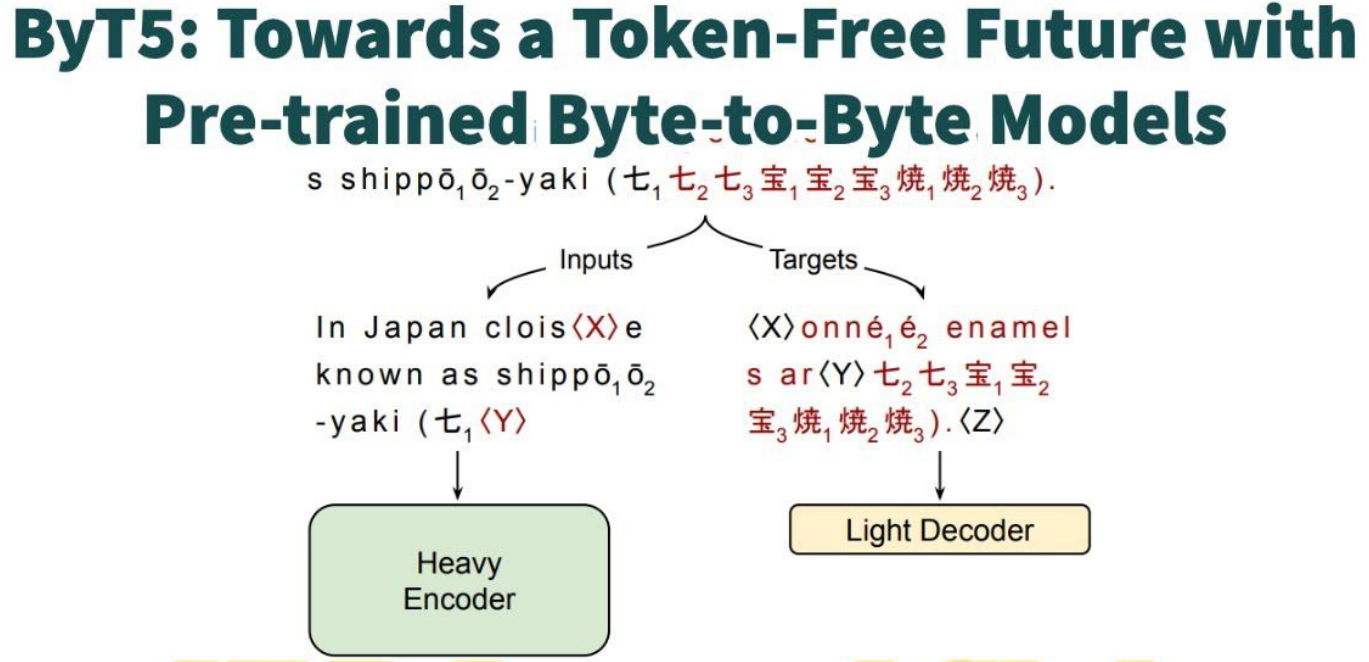
\includegraphics[width=0.60\paperwidth,height=0.60\paperheight,keepaspectratio]{images/large-language-models/llm_byt5_token_free_overview.png}

  {\scriptsize Source: Xue et al., ``ByT5'', TACL 10, 2022, Fig.~1 (right).}
\end{frame}

\begin{frame}{Token-Free LLMs}
  \centering
  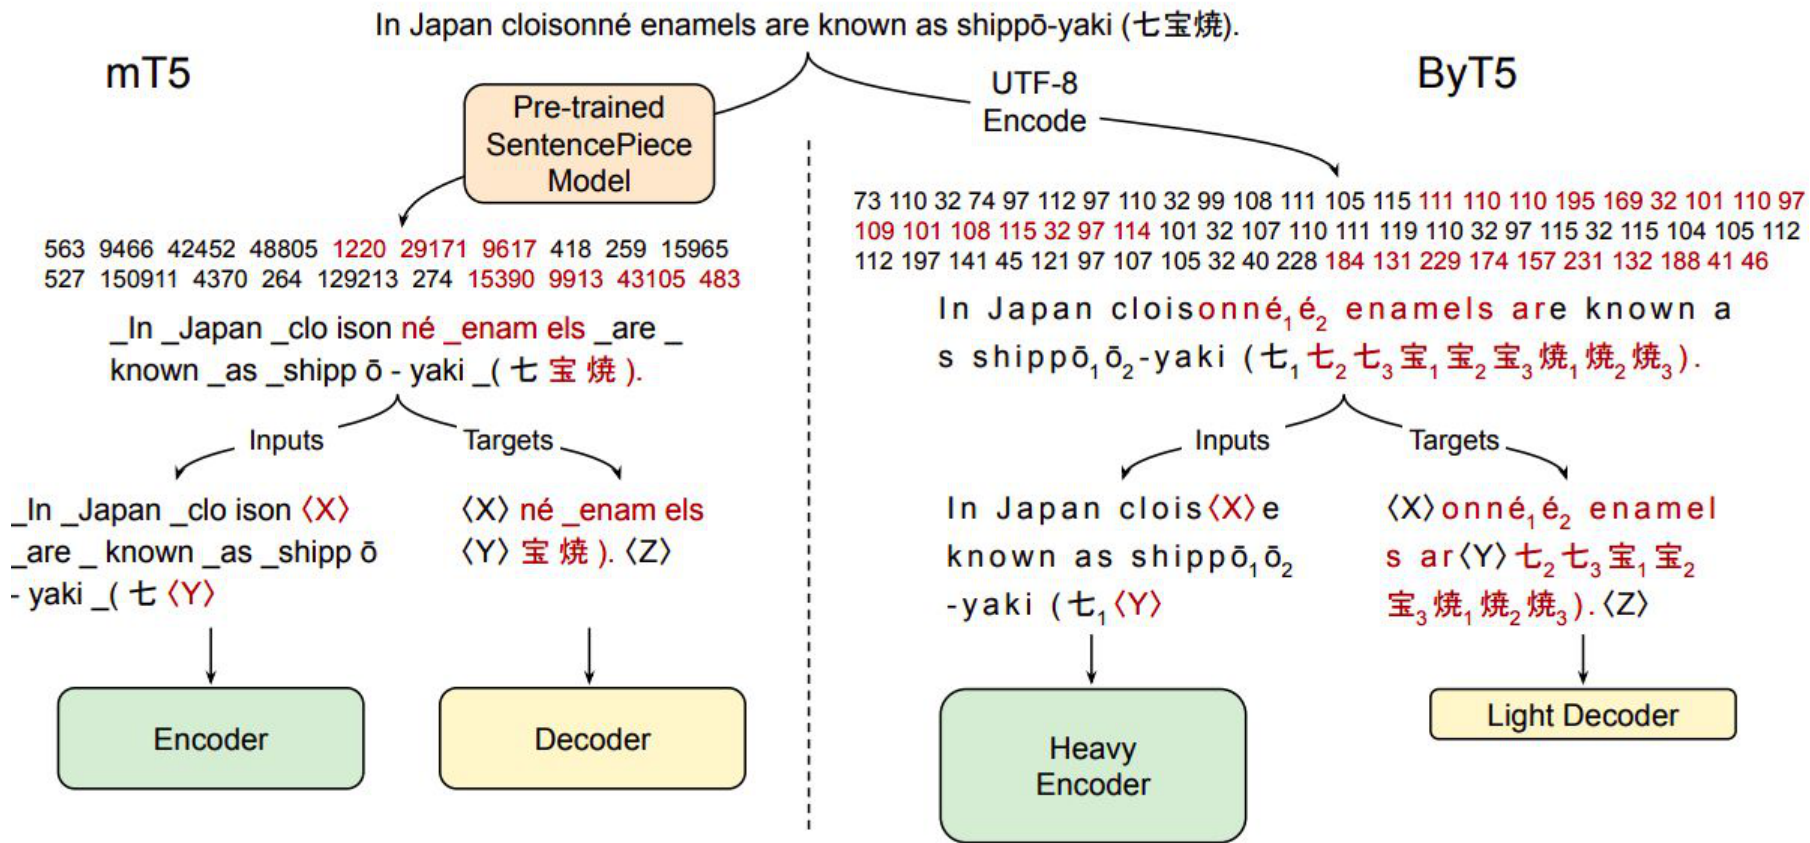
\includegraphics[width=0.60\paperwidth,height=0.60\paperheight,keepaspectratio]{images/large-language-models/llm_mt5_vs_byt5_tokenization.png}

  {\scriptsize Source: Xue et al., ``ByT5'', TACL 10, 2022, Fig.~1.}
\end{frame}

\begin{frame}{Token-Free LLMs}
  \centering
  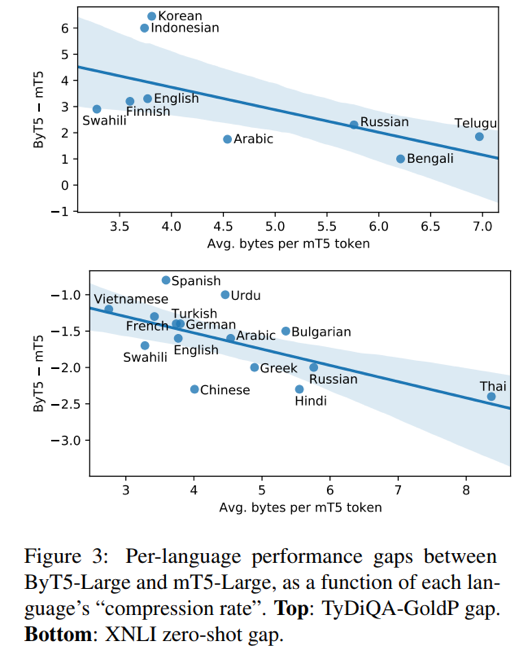
\includegraphics[width=0.8\paperwidth,height=0.75\paperheight,keepaspectratio]{images/large-language-models/llm_byt5_mt5_performance_by_language.png}

  {\scriptsize Source: Xue et al., ``ByT5'', TACL 10, 2022, Fig.~3.}
\end{frame}

\begin{frame}{Token-Free LLMs: Example -- ByT5}
    \small
    \begin{itemize}
        \item \textbf{Example: ByT5 (Xue et al., 2022)}
        \begin{itemize}
            \item Character-level variant of T5 that processes raw bytes instead of tokens.
            \item Eliminates the tokenizer, so any language or script is covered without changing the vocabulary.
        \end{itemize}
        \item \textbf{Pros:}
        \begin{itemize}
            \item No preprocessing or tokenization pipeline required.
            \item Handles any language or script out of the box, with no unknown tokens.
            \item Wins below $\sim$1B parameters, on generative tasks, on spelling-sensitive word-level tasks, and on noisy input.
        \end{itemize}
        \item \textbf{Cons:}
        \begin{itemize}
            \item Training is slower due to longer input sequences.
            \item Increased computational requirements.
            \item mT5 regains the advantage on classification above $\sim$1B parameters.
        \end{itemize}
    \end{itemize}
    {\scriptsize \textbf{Source:} Xue et al., ``ByT5,'' \textit{TACL} 10, 2022, \href{https://arxiv.org/abs/2105.13626}{arXiv:2105.13626}.}
\end{frame}

\begin{frame}{Token-Free LLMs}
  \begin{itemize}
    \item[\textcolor{red}{$\blacktriangleright$}] \textbf{Current Research:}
    \begin{itemize}
      \item Encoders that learn their own segmentation instead of using a fixed vocabulary: \textit{CANINE}, \textit{Charformer}.
      \item Decoders that group bytes into patches to keep sequences short: \textit{MEGABYTE}, \textit{Byte Latent Transformer}.
    \end{itemize}
    \vspace{1em}
    \item[\textcolor{red}{$\blacktriangleright$}] \textbf{Future Directions:}
    \begin{itemize}
      \item Integrating token-free approaches with existing LLMs.
      \item Enhancing efficiency and scalability of token-free models.
    \end{itemize}
  \end{itemize}
\end{frame}
